\documentclass[aspectratio=169]{beamer}
\usetheme{CambridgeUS}

\PassOptionsToPackage{table}{xcolor}
\usepackage{colortbl}
\usepackage{booktabs}
%\usepackage{float}
%\usepackage[table]{xcolor}
%\definecolor{darkgreen}{rgb}{0.0, 0.2, 0.13}
\definecolor{DartmouthGreen}{rgb}{0.05, 0.5, 0.06}
\definecolor{darkred}{rgb}{0.55, 0.0, 0.0}
\definecolor{Crimson}{rgb}{0.86, 0.08, 0.24}
\usepackage{tikz}
%\usetikzlibrary{shadows.blur}
\usetikzlibrary{decorations.pathmorphing}
\usepackage{tikz}
\usepackage{tikz-3dplot}      % simple 3-D perspective
\tdplotsetmaincoords{70}{115} % (elevation, azimuth)

\title{\textbf{Is Pairs Trading a Thing of the Past?}}
\author{\textbf{Jesus Villota Miranda}}
\institute{\textsc{cemfi}}
\date{
32nd Finance Forum 
%$|$ PhD Mentoring Day
%\\ \bigskip
(\today)
}

\AtBeginSection[]{
\begin{frame}{Outline}
\tableofcontents[currentsection]
\end{frame}
}


\begin{document}


\begin{frame}
  \titlepage
\end{frame}

\section{Introduction}
%%%%%%%%%%%%%%%%%%%%%%%%%%%%%%%%%%%%%%%%%%%%%%%%%%%%%
\begin{frame}{History of Pairs Trading}
\begin{itemize}
\item Developed by a group of ``\textit{quants}'' at Morgan Stanley in the 1980s.�
\medskip
\begin{itemize}
\item Pioneered by Gerry Bamberger 
\item Advanced by a team of mathematicians and physicists led by Nunzio Tartaglia
\end{itemize}
\smallskip
\item In 1987, Morgan Stanley  made \$50 mill. on Tartaglia's team's automated systems 
%(an outstanding profit at the time)
\smallskip
\item Although the Morgan Stanley group disbanded in 1989 after a period of performance, \textbf{pairs trading has since become an increasingly popular ``market-neutral'' investment strategy} used by  hedge funds, individual and institutional traders,.
%\item For a considerable time, pairs trading was a closely guarded secret used by Wall Street professionals and institutional investors.�
%\item More hedge funds started to employ this strategy: D.E. Shaw (now TwoSigma) and Long-Term Capital Management
\end{itemize}

\smallskip
\begin{columns}
    \begin{column}{0.2\textwidth}
        \centering
         
\includegraphics[scale=0.22]{/Users/jesusvillotamiranda/Library/CloudStorage/OneDrive-UniversidaddeLaRioja/GitHub/Repository/TeX_Repo/Pairs-Trading-a-Sparse-Synthetic-Control/__presentation__/morgan_stanley.jpg}
    \end{column}
    \begin{column}{0.4\textwidth}
        \centering
        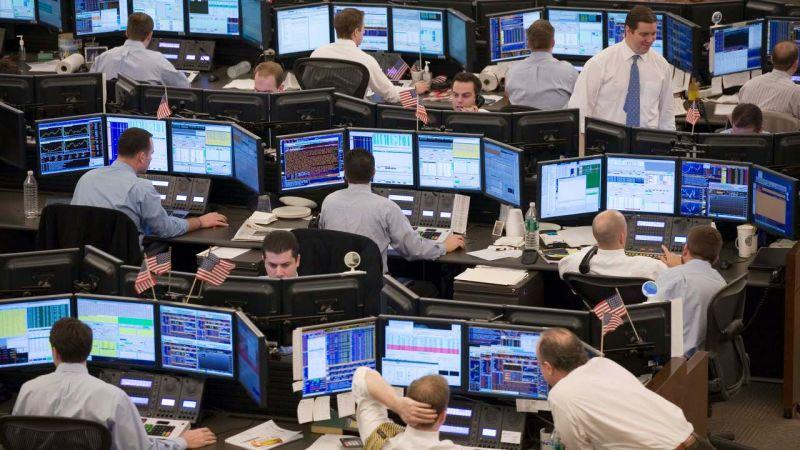
\includegraphics[scale=0.8]{/Users/jesusvillotamiranda/Library/CloudStorage/OneDrive-UniversidaddeLaRioja/GitHub/Repository/TeX_Repo/Pairs-Trading-a-Sparse-Synthetic-Control/__presentation__/trading_floor.jpg}
    \end{column}
\end{columns}


%\begin{center}
%Pairs trading has since become an increasingly popular ``market-neutral'' investment strategy used by hedge funds, individual and institutional traders.
%\end{center}

\end{frame}

%%%%%%%%%%%%%%%%%%%%%%%%%%%%%%%%%%%%%%%%%%%%%%%%%%%%%
\begin{frame}{How the strategy works}
\begin{columns}

% Left column: Explanation
\begin{column}{0.45\textwidth}
\begin{enumerate}
    \item Search for \textbf{two securities} whose \textbf{prices} tend to move together.
\smallskip
    \item Hypothesize that this relationship will hold over time.
\smallskip
    \item When a price \textbf{divergence} occurs, simultaneously:
    \begin{itemize}
        \item \textcolor{DartmouthGreen}{\textsc{long}} the \textcolor{Crimson}{\textsc{underperforming}} security
        \item \textcolor{Crimson}{\textsc{short}} the \textcolor{DartmouthGreen}{\textsc{outperforming}} security
    \end{itemize}
\smallskip
    \item When asset prices \textbf{converge}, close both positions to realize a profit.
\end{enumerate}
\end{column}

% Right column: Figure
\begin{column}{0.55\textwidth}
\centering
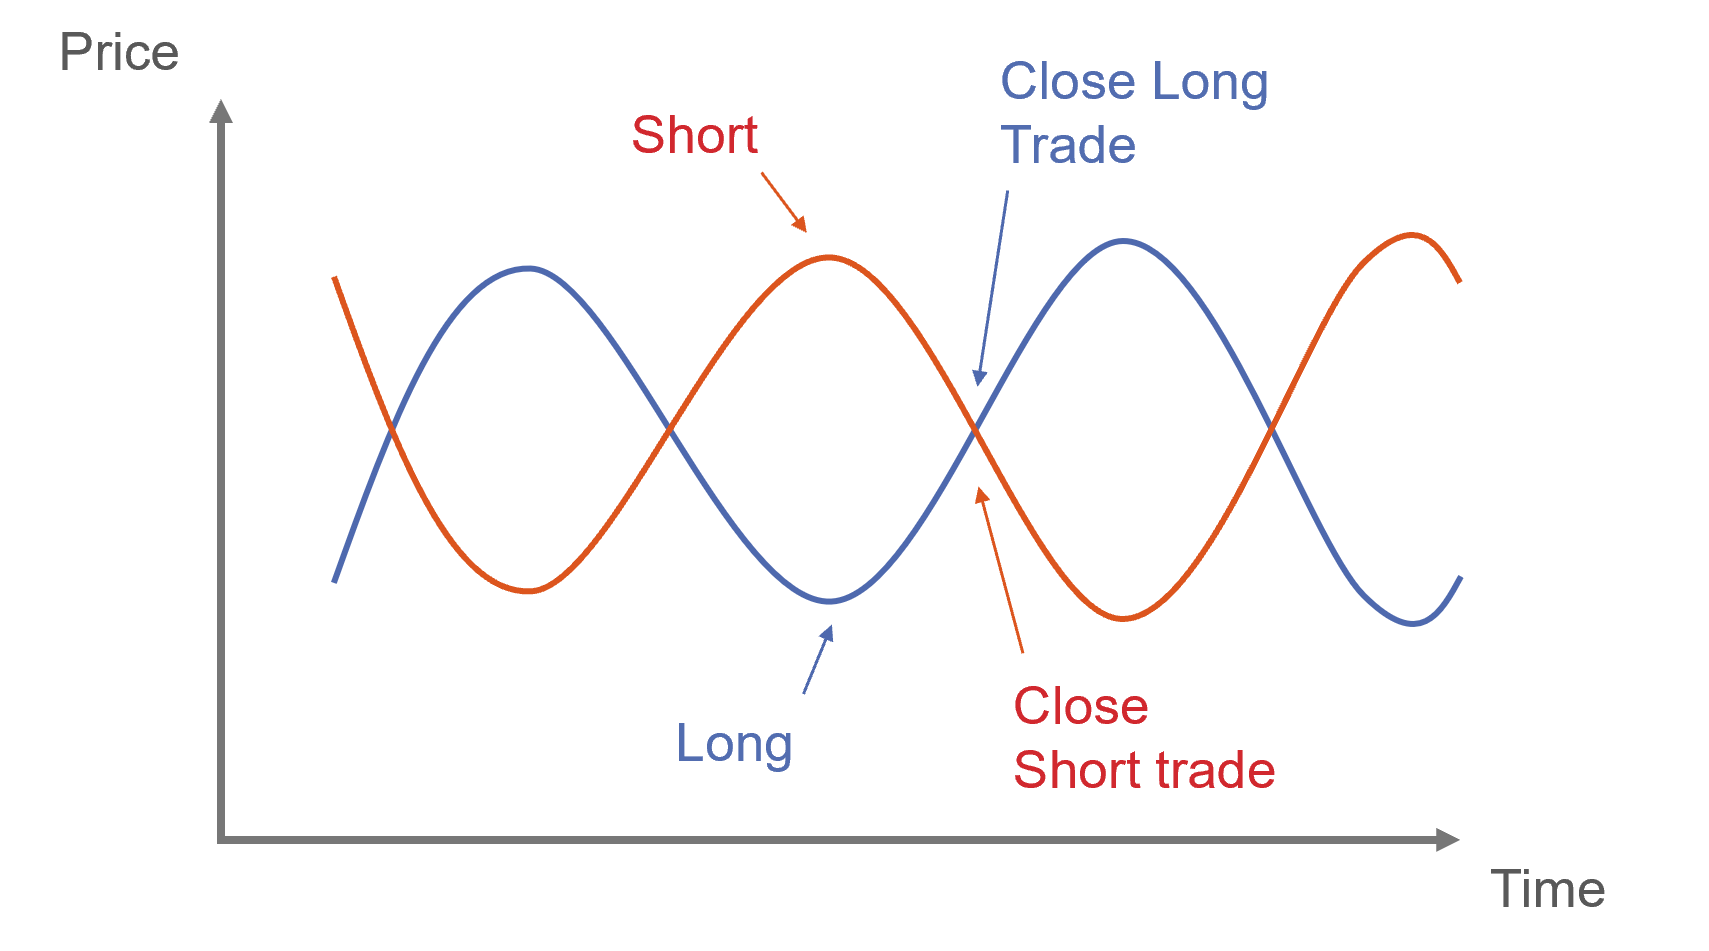
\includegraphics[scale=0.137]{/Users/jesusvillotamiranda/Library/CloudStorage/OneDrive-UniversidaddeLaRioja/GitHub/Repository/TeX_Repo/Pairs-Trading-a-Sparse-Synthetic-Control/__presentation__/taxonomy_pairs_trading.png}
\end{column}

\end{columns}
\end{frame}

%\begin{frame}{How the Strategy Works}
%\begin{enumerate}
%	\item Search for two securities whose prices tend to move together.
%	\item Hypothesize that this relationship will hold over time.
%	\item When a price divergence occurs, simultaneously:
%	\begin{itemize}
%		\item \textcolor{DartmouthGreen}{\textsc{long}} the \textcolor{Crimson}{\textsc{underperforming}} security
%		\item \textcolor{Crimson}{\textsc{short}} the \textcolor{DartmouthGreen}{\textsc{outperforming}} security.
%	\end{itemize}
%\item When asset prices converge, closes both positions to realize a profit
%\end{enumerate}
%
%\begin{figure}[H]
%  \centering
%%  \caption{TBA}
%  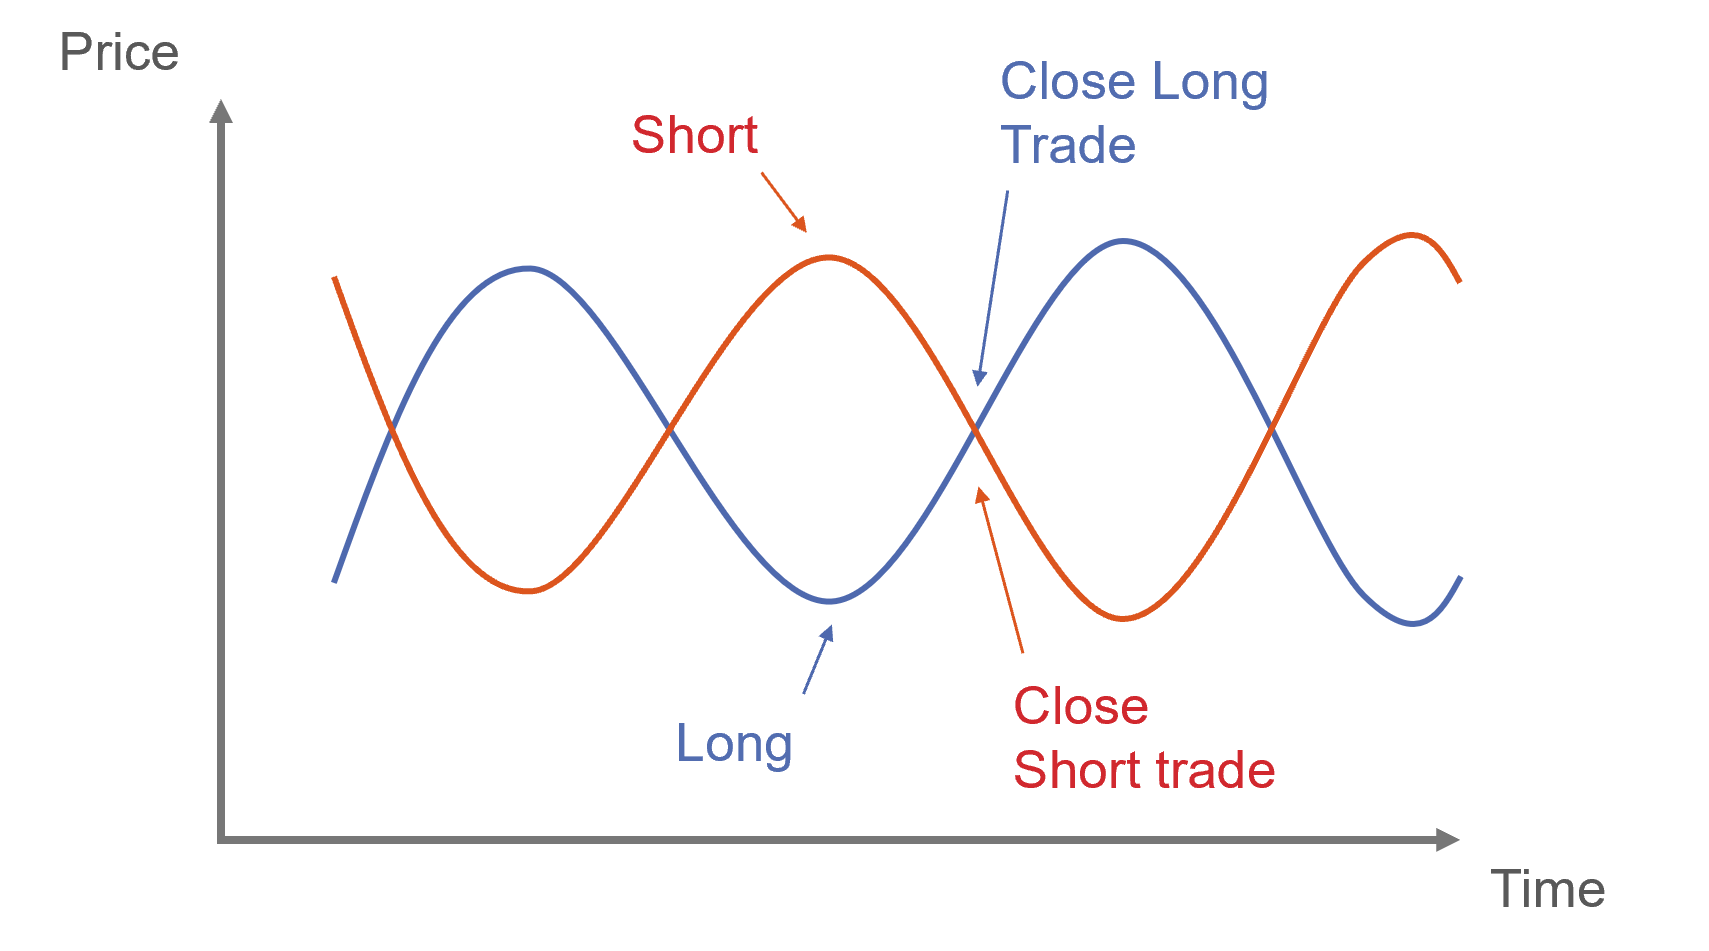
\includegraphics[scale=0.12]{/Users/jesusvillotamiranda/Library/CloudStorage/OneDrive-UniversidaddeLaRioja/GitHub/Repository/TeX_Repo/Pairs-Trading-a-Sparse-Synthetic-Control/__presentation__/taxonomy_pairs_trading.png}
%  \label{fig:}
%\end{figure}
%\end{frame}

%%%%%%%%%%%%%%%%%%%%%%%%%%%%%%%%%%%%%%%%%%%%%%%%%%%%%
\begin{frame}{Theoretical Underpinnings: \textsc{Asset Pricing}}

Asset Pricing can be viewed in \textbf{absolute} and \textbf{relative} terms:


        \begin{itemize} 
        \item \textcolor{blue}{\textbf{Absolute pricing}} $\Rightarrow$ securities are valued from \textbf{fundamentals}, such as disconted future cash flows
        
        \medskip
        \item \textcolor{blue}{\textbf{Relative pricing}} $\Rightarrow$   two securities that are \textbf{close substitutes} for each other should sell for the \textbf{same price} (\textit{it does not say what that price should be!})
        

\begin{itemize}
        \medskip
        \item  The \textbf{L}aw of \textbf{O}ne \textbf{P}rice  is applicable to relative pricing (\textit{even if that price is wrong!})
        
        \medskip
        \item According to Ingersoll (1987), the LOP is the proposition that ``\textit{two investments with the same payoff in every state of nature must have the same current value}''. 

        \medskip
        \item In other words, two securities with the \textbf{same payoffs} in all states of the world should sell for the \textbf{same price}
        \end{itemize}
\end{itemize}
\end{frame}

%%%%%%%%%%%%%%%%%%%%%%%%%%%%%%%%%%%%%%%%%%%%%%%%%%%%%
\begin{frame}{Theoretical Underpinnings: \textsc{Co-Integration}}

\begin{itemize}
        \item Pairs trading can be justified within an \textbf{Equilibrium Asset-Pricing framework with nonstationary common factors}

        \medskip
        \item If the long and short components fluctuate with common nonstationary factors, then the \textbf{prices of the component portfolios} (\textit{aka the spread}) would be \textbf{co-integrated} and the pairs trading strategy would be expected to work.
        
        \medskip 
        \item To interpret a pair $(i,j)$ as co-integrated prices, we need to assume that there exists a \textbf{co-integrating vector that has only two nonzero coordinates}: $$\boldsymbol \alpha = \mathbf e_i - \mathbf e_j$$

%        \smallskip
        \item In that case, the sum or difference of scaled prices will be \textbf{reverting to zero} and a trading rule could be constructed to exploit the expected temporary deviations.
\end{itemize}
\end{frame}

%%%%%%%%%%%%%%%%%%%%%%%%%%%%%%%%%%%%%%%%%%%%%%%%%%%%%%
%\begin{frame}{Conceptual underpinnings of pairs trading}
%
%\textsc{Asset pricing}: 
%\begin{itemize}
%		\item Asset pricing can be viewed in \textsc{absolute} and \textsc{relative} terms:
%		\begin{itemize} 
%		\item \textbf{Absolute pricing}: values securities from fundamentals such as disc. future cash flow
%		\item \textbf{Relative pricing}:  means that two
%securities that are close substitutes for each other should sell for the same price (it does not say what that price will be)
%		\item  The \textbf{L}aw of \textbf{O}ne \textbf{P}rice  is applicable to relative pricing, even if that price is wrong.
%\begin{itemize}
%		\item According to Ingersoll (1987), the LOP is the proposition that ``two investments with the same payoff in every state of nature must have the same
%current value''. 
%		\item In other words, two securities with the same prices in all
%states of the world should sell for the same amount
%		\end{itemize}
%\end{itemize}
%\bigskip
%
%	\item \textsc{Co-integration}: 
%\begin{itemize}
%	\item The pairs trading strategy can be justified within an equilibrium asset-pricing framework with nonstationary common factors
%	\item If the long and short components fluctuate with common nonstationary factors, then the prices of the component portfolios would be co-integrated and the pairs trading strategy would be expected to work.
%\end{itemize}
%\end{itemize}
%\end{frame}

%%%%%%%%%%%%%%%%%%%%%%%%%%%%%%%%%%%%%%%%%%%%%%%%%%%%%
\begin{frame}{Literature Review}
    \begin{itemize}
        \item \textbf{[Gatev, Goetzmann, \& Rouwenhorst (GGR), 2006]}
        \begin{itemize}
            \item Their paper, \textit{``Pairs Trading: Performance of a Relative-Value Arbitrage Rule''} is the most-cited and seminal work in the literature.
            \smallskip
            \item First circulated as a working paper in 1999 and later published in the \textit{Review of Financial Studies} (2006).
            \smallskip
            \item It provided the \textbf{first large-scale, rigorous empirical evidence of the strategy's historical profitability}, establishing it as a legitimate field of study.
        \end{itemize}
        
        \bigskip % Adds some vertical space between the two main points
        
        \item \textbf{\cite{Do2010}}
        \begin{itemize}
            \item In their \textit{Financial Analysts Journal} article, they re-examined the GGR strategy with an extended dataset running through 2009.
            \smallskip
            \item They confirmed that profitability was steadily \textbf{decaying}, likely due to the strategy's popularity and increasing market efficiency.
            \smallskip
            \item However, they also discovered that profits temporarily \textbf{resurged} during periods of market turmoil, such as the 2008 Global Financial Crisis (GFC).
        \end{itemize}
    \end{itemize}
\end{frame}

%%%%%%%%%%%%%%%%%%%%%%%%%%%%%%%%%%%%%%%%%%%%%%%%%%%%%
\begin{frame}{The Decay of Pairs Trading}
\begin{figure}[H]
  \caption{Monthly excess returns to Pairs Trading }
  \centering
  \includegraphics[scale=0.4]{/Users/jesusvillotamiranda/Library/CloudStorage/OneDrive-UniversidaddeLaRioja/GitHub/Repository/pairs_trading_sparse_synthetic_replica/__OUTPUT__/figures/pairs_trading_decay.pdf}
  \label{fig:}
\end{figure}
\end{frame}

%%%%%%%%%%%%%%%%%%%%%%%%%%%%%%%%%%%%%%%%%%%%%%%%%%%%%
\begin{frame}{The Decay of Pairs Trading}
\begin{itemize}
\item The \textbf{popularization} of PT has led to a significant \textbf{decline in profitability}
%\begin{itemize}
%    \item Widespread adoption has eroded arbitrage opportunities
%%    \item Market efficiency improvements have reduced persistent mispricings
%\end{itemize}

\medskip
\item However, this decay \textbf{does not invalidate} the underlying principle of {\textbf{relative-value arbitrage}}

%\medskip
%\item The core insight remains powerful: assessing security values relative to close substitutes

\medskip
\item The issue may lie in the \textcolor{darkred}{\textbf{restrictive nature}} of traditional \textcolor{darkred}{\textbf{1-to-1 pairing}}:
\begin{itemize}
    \item Modern markets are \textbf{increasingly efficient}
    \item Simple, stable relationships between individual stocks have become \textbf{scarce}
    \item Traditional pairwise constraints may be \textbf{too limiting}
\end{itemize}
\end{itemize}

\medskip
\begin{center}
\colorbox{DartmouthGreen!20}{%
    \begin{minipage}{0.95\textwidth}
        \centering
        \textcolor{DartmouthGreen}{\textbf{Challenge}}: Identifying more \textbf{robust substitutes} in an increasingly efficient market
    \end{minipage}
}
\end{center}
\end{frame}

%%%%%%%%%%%%%%%%%%%%%%%%%%%%%%%%%%%%%%%%%%%%%%%%%%%%%
\begin{frame}{Recent Literature on Pairs Trading}
\begin{itemize}
    \item The pairs trading literature has \textcolor{darkred}{\textbf{stagnated conceptually}} since GGR
    
    \medskip
    \item Research focus has shifted toward \textbf{methodological refinements} rather than fundamental innovation:
    \begin{itemize}
        \item Advanced statistical techniques for pair identification
        \item Sophisticated modeling of joint stock behavior  
        \item Complex signal generation and position sizing methods
    \end{itemize}
    
    \medskip
    \item This has produced a \textbf{fragmented literature} with several concerning patterns:
    \begin{itemize}
        \item \textcolor{darkred}{\textbf{Incremental improvements}} without clear theoretical justification
        \item \textcolor{darkred}{\textbf{Method selection bias}} - unclear why specific techniques are chosen
        \item \textcolor{darkred}{\textbf{Publication bias}} - potential cherry-picking of favorable results
    \end{itemize}
\end{itemize}

\begin{center}
\colorbox{DartmouthGreen!20}{%
    \begin{minipage}{0.9\textwidth}
        \centering
        \textcolor{DartmouthGreen}{\textbf{Need for:}} \textbf{principled evolution} of the traditional PT framework
    \end{minipage}
}
\end{center}
\end{frame}

%%%%%%%%%%%%%%%%%%%%%%%%%%%%%%%%%%%%%%%%%%%%%%%%%%%%%
\begin{frame}[plain]
%\begin{frame}{Recent Literature}
\begin{tikzpicture}[remember picture, overlay]

% We'll define a style for the paper titles. This makes the code
% much cleaner and easier to modify later.
\tikzset{paper/.style={
    fill=white,           % Add a white background to each title.
    draw=black!20,        % Add a very light gray border.
    rounded corners=3pt,  % Make the corners of the "paper" slightly rounded.
    align=center,         % Center the text inside the node.
    font=\small,          % You can adjust font size here, e.g., \footnotesize, \normalsize.
    text width=4.5cm,     % Set a max width to control line breaking for long titles.
    inner sep=5pt,        % Add some padding between the text and the border.
    fill opacity=0.9,     % Make the background mostly opaque to hide text underneath.
    text opacity=1,       % Ensure the text itself is fully opaque.
%    drop shadow,          % Add a subtle shadow for a 3D/depth effect.
}}

\pgfmathsetseed{44444444}

\foreach \i/\title in {
  1/{Pairs Trading via Unsupervised Learning},
  2/{Structural Break-Aware Pairs Trading via Deep Reinforcement Learning},
%  3/{Statistical Arbitrage in Multi-Pair Trading using Graph Clustering Algorithms},
  4/{Pairs Trading Optimization using Reinforcement Learning and Cointegration},
  5/{Cryptocurrency Pair Forecasting with Machine and Deep Learning},
  6/{Pairs Trading: A Copula Approach},
  7/{A Pairs Trading Strategy Based on Mixed Copulas},
  8/{Profitability of Pairs Trading: Distance, Cointegration \& Copula Methods},
  9/{Black-Litterman Bayesian Application in Statistical Arbitrage},
% 10/{Novel NSGA-II Based Pairs Trading in Crypto Markets},
 11/{Walk-Forward Optimized Forex Cointegration Strategy},
 12/{Hidden Markov Model for Statistical Arbitrage in Oil Futures},
 13/{Pair Trading Based on Quantile Forecasting of Smooth Transition GARCH Models},
% 14/{A Singular Stochastic Control Approach for Optimal Pairs Trading with Proportional Transaction Costs},
 15/{An Intelligent Model for Pairs Trading Using Genetic Algorithms},
 16/{Pairs Trading with Wavelet Transform},
 17/{Dynamic Copula Framework for Pairs Trading},
 18/{Cointegration Approach for the Pair Trading Based on the Kalman Filter},
 19/{Pairs Trading with a Mean-Reverting Jump-Diffusion Model on High-Frequency Data},
 20/{Review of Stochastic Differential Equations in Statistical Arbitrage Pairs Trading},
% 21/{A Singular Stochastic Control Approach for Optimal Pairs Trading with Proportional Transaction Costs},
 22/{Pairs Trading with Markov Regime-Switching Model},
 23/{Research on High-Frequency Stock Pair Trading Strategy Based on MS-GARCH Model}
}{
  % Use page dimensions for better random placement across the whole slide.
  % 'rnd' is a random number between 0 and 1.
  \pgfmathsetmacro\x{rnd * 0.8 * \paperwidth - 0.4 * \paperwidth}
  \pgfmathsetmacro\y{rnd * 0.7 * \paperheight - 0.35 * \paperheight}

  % Use a more subtle rotation to improve readability.
  \pgfmathsetmacro\r{rnd * 12 - 6} % Rotates between -6 and +6 degrees.

  % Apply the 'paper' style to the node.
  \node[paper, rotate=\r] at ([xshift=\x, yshift=\y]current page.center) {\title};
}

% Optional: You could add a main title in the center so it stands out.
\node[font=\Huge\bfseries, text=black!60] at (current page.center) {Pairs Trading};

\end{tikzpicture}
\end{frame}

%%%%%%%%%%%%%%%%%%%%%%%%%%%%%%%%%%%%%%%%%%%%%%%%%%%%%
%\begin{frame}{Literature Review}
%	\begin{itemize}
%	\item In 1998, Gatev, Goetzmannet and Rouwenhorst released their wroking paper ``\textit{Pairs trading: Performance of a relative-value arbitrage rule}''. 
%	\item In 2006, this paper is published in the Review of Financial Studies (2006)
%	\item This is the most-cited and reference paper in the pairs trading literature
%	\item In 2010, Do and Faff (2010, \textit{FAJ}) review this paper extending the dataset to 2010 and show that protiability is dcaying, but that it goes up during the GFC
%\end{itemize}
%\end{frame}

%%%%%%%%%%%%%%%%%%%%%%%%%%%%%%%%%%%%%%%%%%%%%%%%%%%%%
%\begin{frame}{Recent literature on pairs trading}
%\begin{itemize}
%	\item The literature on pairs trading hasn't conceptually evolved since Gatev et al's seminal paper
%	\item Instead, reserachers have focused on ``improving'' (applying more sophisticated methods) to the original strategy
%	\item The result has been a bast body of research with fancy titles looking at very specific elements of the strategy and claiming to improve it.
%	\item Many of these papers do not provide a clear justification for why a particular for, say, finding pairs, or modeling the joint behavior of stocks, is better over others.
%	\item Many authors don't justify why we should choose these methods: in other words,  it's not clear whether these methods are cherry-picked to look good for publication.
%\end{itemize}
%\end{frame}

%%%%%%%%%%%%%%%%%%%%%%%%%%%%%%%%%%%%%%%%%%%%%%%%%%%%%%
%\begin{frame}{This paper}
%
%\begin{center}
%Is this one more paper in this ocean of pairs trading papers?
%\end{center}
%
%\begin{itemize}
%	\item Hopefully not. 
%	\item In this paper I try to make a small advancement in the conception of ``pairs trading'' with a very simple idea. 
%	\item Why rely on a single asset to find the substitute of a target asset?
%	\item Wouldn't it be better to use..., say... a combination of assets?
%	\item That's the simple idea behind this paper
%	\item We will find substitutes by creating a replicating portfolio of the target asset
%\end{itemize}
%\end{frame}

%%%%%%%%%%%%%%%%%%%%%%%%%%%%%%%%%%%%%%%%%%%%%%%%%%%%%
\begin{frame}{Can we reframe the idea of Pairs Trading?}

\textbf{The Limitation of the Traditional Approach}
\begin{itemize}
\item Traditional pairs trading imposes a \textcolor{darkred}{\textbf{severe cardinality constraint}}:
\begin{itemize}
    \item Limited to finding \textbf{one single substitute} security for any target asset
    \item While conceptually elegant, this restriction may be \textcolor{darkred}{\textbf{unnecessarily limiting}} in practice
\end{itemize}
\end{itemize}

\bigskip 
\textbf{A More Flexible Approach}
\begin{itemize}
\item  Instead of searching for one perfect substitute, why not construct a \textbf{synthetic replica} using multiple securities?

\medskip
\item \textbf{Example - General Motors}: Rather than finding a single stock that tracks GM's movements:
\begin{itemize}
    \item Use a \textbf{linear combination} of multiple securities
    \item Create a more accurate synthetic substitute  
    \item Capture complex relationships that no single stock can replicate
\end{itemize}
\end{itemize}

\medskip
\begin{center}
\colorbox{DartmouthGreen!20}{%
    \begin{minipage}{0.95\textwidth}
        \centering
        \textcolor{DartmouthGreen}{\textbf{Key Idea}}: We can generalize the search for substitutes from \textbf{1-to-1} to \textbf{1-to-\textit{portfolio}}
%        while preserving the relative-value arbitrage principle
    \end{minipage}
}
\end{center}

\end{frame}

%%%%%%%%%%%%%%%%%%%%%%%%%%%%%%%%%%%%%%%%%%%%%%%%%%%%%%
%\begin{frame}{Can we reframe the idea of Pairs Trading?}
%\begin{itemize}
%\item Traditional pairs trading imposes a severe cardinality constraint by limiting the replication of a target asset to a single substitute security. 
%\item This restriction, while conceptually elegant, may be unnecessarily limiting in practice. 
%\item Consider General Motors: rather than searching for a single stock whose normalized price series closely tracks GM's movements, we could construct a synthetic replica using a linear combination of multiple securities. 
%\item This approach maintains the fundamental economic intuition of pairs trading--exploiting temporary deviations between economically related assets--while providing greater flexibility in replica construction.
%\end{itemize}
%\end{frame}

%%%%%%%%%%%%%%%%%%%%%%%%%%%%%%%%%%%%%%%%%%%%%%%%%%%%%
%\begin{frame}{Generalizing Pairs Trading: A Replicating Portfolio approach}
%\begin{itemize}
%\item The theoretical foundation remains rooted in relative pricing theory, where securities serving as close economic substitutes should exhibit similar price dynamics. However, our framework relaxes the stringent requirement that such substitution be achieved through a single asset. Instead, we allow for the construction of synthetic substitutes through sparse linear combinations, potentially improving the replication of the target asset.
%
%\item This paper proposes a generalization of the pairs trading framework that relaxes this rigid cardinality constraint. Instead of searching for a single, naturally occurring substitute for a target asset, we propose to construct a ``synthetic replica'' of it. Methodologically, this is achieved by regressing the normalized price series of the target asset against a broad ``donor pool'' of potential substitutes. The fitted values from this regression form the price series of the synthetic replica --a portfolio of assets weighted to best track the target. The spread in this generalized framework is therefore the regression error: the price difference between the target asset and its synthetic replica. 
%\end{itemize}
%\end{frame}


%%%%%%%%%%%%%%%%%%%%%%%%%%%%%%%%%%%%%%%%%%%%%%%%%%%%%
%\begin{frame}{Generalizing Pairs Trading: A Replicating Portfolio Approach}
%
%%\textbf{Core Innovation:} Relaxing the \textcolor{darkred}{\textbf{single-asset constraint}}
%
%\medskip
%\begin{columns}
%    \begin{column}{0.4\textwidth}
%        \textcolor{blue}{\textbf{Traditional Approach}}
%        \begin{itemize}
%            \item One target asset
%            \item One substitute asset
%            \item Rigid 1-to-1 pairing
%        \end{itemize}
%    \end{column}
%    \begin{column}{0.4\textwidth}
%        \textcolor{DartmouthGreen}{\textbf{Replicating Portfolio Approach}}
%        \begin{itemize}
%            \item One target asset
%            \item \textbf{Portfolio} of substitutes
%            \item Flexible replication
%        \end{itemize}
%    \end{column}
%\end{columns}
%
%\bigskip
%\bigskip
%
%\textbf{Modus Operandi:}
%\begin{enumerate}
%    \item Regress target asset against a \textbf{``donor pool''} of potential substitutes
%    \item Fitted values create a \textcolor{DartmouthGreen}{\textbf{replicating portfolio}}
%    \item Trade the spread between target and its replicating portfolio
%\end{enumerate}
%
%\end{frame}
%\medskip
%\begin{center}
%\colorbox{DartmouthGreen!20}{%
%    \begin{minipage}{0.9\textwidth}
%        \centering
%        \textcolor{DartmouthGreen}{\textbf{Key Advantage}}: Maintains relative pricing theory while enabling \textbf{better replication}
%    \end{minipage}
%}
%\end{center}




\begin{frame}{Generalizing Pairs Trading: a Replicating Portfolio Approach}

\begin{columns}[T] % The [T] option aligns the content at the top

    \begin{column}{0.48\textwidth}
        \begin{beamercolorbox}[sep=0.8em,center]{titlelike}
            \textbf{Traditional Approach}
        \end{beamercolorbox}
        \begin{itemize}
            \item \textbf{Structure:} Rigid 1-to-1 pairing.
            \medskip
            \item \textbf{Substitute:} A single, similar stock.
            \medskip
            \item \textbf{Spread:} Price(A) - Price(B).
            \medskip
            \item \textbf{Limitation:} Stable, reliable pairs are now scarce.
        \end{itemize}
    \end{column}

%    \pause % This will reveal the second column after a click

    \begin{column}{0.48\textwidth}
        \begin{beamercolorbox}[sep=0.8em,center]{titlelike}
            \textbf{Replicating Portfolio Approach}
        \end{beamercolorbox}
        \begin{itemize}
            \item \textbf{Structure:} Flexible 1-to-many.
            \medskip
            \item \textbf{Substitute:} A \textbf{synthetic replica} (a portfolio).
            \medskip
            \item \textbf{Spread:} Price(Target) - Price(Replica).
            \medskip
            \item \textbf{Advantage:} More robust and flexible replication.
        \end{itemize}
    \end{column}

\end{columns}

\vfill % Pushes the following content to the bottom of the slide

\medskip 
\begin{center}
\colorbox{DartmouthGreen!20}{%
    \begin{minipage}{0.95\textwidth}
        \centering
        Our approach preserves the same Asset pricing and Cointegration underpinnings as traditional PT
    \end{minipage}
}
\end{center}

\end{frame}

\section{Methodology}
%%%%%%%%%%%%%%%%%%%%%%%%%%%%%%%%%%%%%%%%%%%%%%%%%%%%%
\begin{frame}{Pairs Trading as a Replicating Portfolio problem}
\begin{itemize}
\item The economic intuition behind pairs trading --exploit temporary mispricing between two close substitutes-- can be cast more generally as a problem of \emph{relative valuation}.  

\medskip
\item Rather than forcing the substitute for a target stock $i$ to be a \emph{single} partner, we allow it to be a \emph{replicating portfolio}: a linear combination of securities whose joint price path mimics that of $i$.
%----------------------------------------------------
\begin{equation} \label{eq:regression}
p_{i,t}= \sum_{j\in\mathcal D} \beta_j\,p_{j,t}+ \varepsilon_{i,t},
\qquad t=0,\dots,T ,
\end{equation}
%----------------------------------------------------
where:
\begin{itemize}
\item $p_{i,t}$ represents the \textit{normalized price} (i.e.: cumulative return) of the target asset
%\footnote{
%The normalized price time series of a stock $i$ is built from a position where 1 dollar is invested at the beginning of the estimation window. Formally, letting $r_{i,0}=0$, the normalized price time series at time $t$ is:
%$$
%p_{i,t} = \prod_{\tau=0}^t (1+r_{i,\tau} )
%$$
%}, 
\item $\mathcal{D}$ denotes the donor pool of potential replicating assets, and 
\item $\varepsilon_{i,t}$ denotes the spread between the target and its synthetic replica. 
\end{itemize}

%Traders should then be interested in trading the spread between the target stock and the replicating portfolio, which is simply the residual error $\varepsilon_{i,t}$, by betting on its mean-reversion. 
%
%While \cref{eq:general_reg} describes the unrestricted case, where no structure is imposed in the replicating portfolio, we can show that a restricted version from this general framework delivers the classical pairs trading methodology. 
\end{itemize}
\end{frame}

%%%%%%%%%%%%%%%%%%%%%%%%%%%%%%%%%%%%%%%%%%%%%%%%%%%%%
\begin{frame}{Recasting Gatev's Pairs Trading as a Replicating Portfolio problem}

Note that traditional pairs trading, as described in Gatev et al, is a special case where the regression coefficient vector is restricted to the canonical basis. 
\bigskip 

\begin{itemize}
%\begin{itemize}
\item Let $\mathcal B:=\{\mathbf e_1,\mathbf e_2,\dots,\mathbf e_{|\mathcal D|}\}$, denote the canonical basis of $\mathbb R^{|{\mathcal D}|}$. 

\bigskip
\item ``Traditional'' pairs trading fixes a target stock $i$ and selects a single-asset replicating portfolio in a 1-to-1 relationship by imposing the restriction $\boldsymbol \beta \in \mathcal B$.
%\end{itemize}
%------------------------------------------
\begin{align*}
%&
%\underset{\boldsymbol \beta\in\mathcal B}{\min}
\min_{\boldsymbol \beta\in\mathcal B}{~
        \sum_{t=0}^{T}
        \Bigl(p_{i,t}-\sum_{j\in\mathcal D}\beta_j p_{j,t}\Bigr)^2
        }
\end{align*} 
%----------------------------------------------------
\end{itemize}
\end{frame}


%%%%%%%%%%%%%%%%%%%%%%%%%%%%%%%%%%%%%%%%%%%%%%%%%%%%%
\begin{frame}
\begin{itemize}
\item ``Traditional'' pairs trading fixes a target stock $i$ and selects a single-asset replicating portfolio in a 1-to-1 relationship by imposing the restriction $\boldsymbol \beta \in \mathcal B$.
%\end{itemize}
%------------------------------------------
\begin{align*}\label{eq:choose_pair}
%&
%\underset{\boldsymbol \beta\in\mathcal B}{\min}
\min_{\boldsymbol \beta\in\mathcal B}{~
        \sum_{t=0}^{T}
        \Bigl(p_{i,t}-\sum_{j\in\mathcal D}\beta_j p_{j,t}\Bigr)^2
        }
\end{align*} 
%----------------------------------------------------

%\bigskip
\item Under this formulation, the only nonzero element of the coefficient vector will correspond to that of the \textbf{stock} whose \textbf{price} series \textbf{minimizes} the \textbf{least-squares (or euclidean) distance} \textbf{with respect to that of the target stock}. 
%----------------------------------------------------
\begin{align}
j^*
= 
\arg \min_{j\in\mathcal D}{~
        \sum_{t=0}^{T}
        \bigl(p_{i,t}-p_{j,t}\bigr)^2
        } 
\end{align}
%----------------------------------------------------
\end{itemize}
\end{frame}


%%%%%%%%%%%%%%%%%%%%%%%%%%%%%%%%%%%%%%%%%%%%%%%%%%%%%
\begin{frame}
\begin{itemize}
\item Note that pairs trading with a hedge ratio is equivalent to restricting $\boldsymbol \beta$ to lie in $\mathcal B^+:=\{
\alpha \mathbf e_j : j\in \mathcal D, \alpha\in\mathbb R
\}$. Hence:
$$
\begin{array}{l}
\underset{\boldsymbol \beta\in\mathcal B^+}{\min}
        \sum_{t=0}^{T}
        \Bigl(p_{i,t}-\sum_{j\in\mathcal D}\beta_j p_{j,t}\Bigr)^2
\end{array}
%\right]
$$

\bigskip
\item Which is equivalent to choosing $\boldsymbol \beta$ freely but imposing unit cardinality in the coefficient vector 
$$ 
\begin{array}{rl}
\underset{\boldsymbol \beta\in\mathbb R^{|{\mathcal D}|}}{\min}
& \sum_{t=0}^{T} \Bigl(p_{i,t}-\sum_{j\in\mathcal D}\beta_j p_{j,t}\Bigr)^2
\\
\mathrm{s.t.} & \lVert{\boldsymbol{\beta}\rVert}_0 = 1
\end{array}
$$
\end{itemize}
\end{frame}


%%%%%%%%%%%%%%%%%%%%%%%%%%%%%%%%%%%%%%%%%%%%%%%%%%%%%
%%%%%%%%%%%%%%%%%%%%%%%%%%%%%%%%%%%%%%%%%%%%%%%%%%%%%
\begin{frame}{Canonical vs.\ Augmented Canonical Space}
\begin{columns}[c]
%-----------------------------------------------------------------
% RIGHT :  Ordinary 3-D canonical basis  {e1,e2,e3}
%-----------------------------------------------------------------
\begin{column}{0.48\textwidth}
\centering
\begin{tikzpicture}[scale=1.45,tdplot_main_coords,>=stealth]

% axes -----------------------------------------------------------
\draw[->,thin] (0,0,0) -- (2.5,0,0) node[anchor=north east] {$x_1$};
\draw[->,thin] (0,0,0) -- (0,2,0) node[anchor=north west] {$x_2$};
\draw[->,thin] (0,0,0) -- (0,0,2) node[anchor=south]     {$x_3$};

% unit vectors ---------------------------------------------------
\draw[very thick,Crimson,->]          (0,0,0) -- (1.8,0,0);
\draw[very thick,DartmouthGreen,->]   (0,0,0) -- (0,1.5,0);
\draw[very thick,blue,->]             (0,0,0) -- (0,0,1.5);

% e_1 label, offset to avoid overlap
\node[Crimson, font=\small, anchor=south west] at (1.8,0.4,0) {$\mathbf{e}_1$};
% e_2 label
\node[DartmouthGreen, font=\small, anchor=south east] at (0,1.3,0) {$\mathbf{e}_2$};
% e_3 label
\node[blue, font=\small, anchor=south west] at (0,0,1) {$\mathbf{e}_3$};

\end{tikzpicture}

% Caption below the figure
\vspace{0.5em}
{\footnotesize
$\mathcal{B} = \left\{ \mathbf{e}_1,\,\mathbf{e}_2,\,\mathbf{e}_3 \right\}$
}

\end{column}

%-----------------------------------------------------------------
% LEFT  :  "Augmented" canonical vectors  (all possible scalings)
%-----------------------------------------------------------------
\begin{column}{0.48\textwidth}
\centering
\begin{tikzpicture}[scale=1.45,tdplot_main_coords,>=stealth]

% axes -----------------------------------------------------------
\draw[->,thin] (-2,0,0) -- ( 2,0,0) node[anchor=north east] {$x_1$};
\draw[->,thin] ( 0,-2,0) -- ( 0,2,0) node[anchor=north west] {$x_2$};
\draw[->,thin] ( 0,0,-2) -- ( 0,0,2) node[anchor=south]     {$x_3$};

% "rays" generated by the canonical basis ------------------------
\foreach \s in {0.4,0.8,1.2,1.6}{
  %  e_1 - red  ---------------------------------------------------
  \draw[very thick,Crimson,->]          (0,0,0) -- ( \s,0,0);
  \draw[very thick,Crimson!50!black,->] (0,0,0) -- (-\s,0,0);
  %  e_2 - green -------------------------------------------------
  \draw[very thick,DartmouthGreen,->]          (0,0,0) -- (0, \s,0);
  \draw[very thick,DartmouthGreen!50!black,->] (0,0,0) -- (0,-\s,0);
  %  e_3 - blue  -------------------------------------------------
  \draw[very thick,blue,->]          (0,0,0) -- (0,0, \s);
  \draw[very thick,blue!50!black,->] (0,0,0) -- (0,0,-\s);
}

% e_1 label, offset to avoid overlap
\node[Crimson, font=\small, anchor=south west] at (1.6,-0.45,0) {$\alpha\mathbf{e}_1$};
% e_2 label
\node[DartmouthGreen, font=\small, anchor=south east] at (0,1.6,0.1) {$\alpha\mathbf{e}_2$};
% e_3 label
\node[blue, font=\small, anchor=south west] at (0,0,1.1) {$\alpha\mathbf{e}_3$};

\end{tikzpicture}

% Caption below the figure
\vspace{0.5em}
{\footnotesize
$\mathcal{B}^{+} = \left\{ \alpha\,\mathbf{e}_i : \alpha\in\mathbb{R},\; i=1,2,3 \right\}$
}

\end{column}



\end{columns}
\end{frame}
%%%%%%%%%%%%%%%%%%%%%%%%%%%%%%%%%%%%%%%%%%%%%%%%%%%%%



%%%%%%%%%%%%%%%%%%%%%%%%%%%%%%%%%%%%%%%%%%%%%%%%%%%%%
\begin{frame}{Pairs Trading a Sparse Replicating Portfolio} 
\begin{itemize}
\item We avoid imposing such restrictive cardinality restrictions, and allow for a denser regression coefficient vector. However, we deliberately promote sparsity to avoid excessive transaction costs. 


\bigskip
\item For this purpose, we employ the LASSO regularization [Tibshirani, 2006]
%----------------------------------------------------
\begin{align}
\label{eq:lasso}
\min_{\boldsymbol \beta \in \mathbb R^{|{\mathcal D}|}} 
\left\{ 
\sum_{t=0}^T 
\Bigl( 
p_{i,t} - \sum_{j \in \mathcal{D}} \beta_j p_{j,t} 
\Bigr)^2 
+ 
\lambda \sum_{j \in \mathcal{D}} |\beta_j| 
\right\}
\end{align}
%----------------------------------------------------
\end{itemize}
\end{frame}

%%%%%%%%%%%%%%%%%%%%%%%%%%%%%%%%%%%%%%%%%%%%%%%%%%%%%
\begin{frame}{Replicating Portfolio Approach: Any Vector in \(\mathbb{R}^3\)}
\centering
\begin{tikzpicture}[scale=1.5,tdplot_main_coords,>=stealth]

% axes
\draw[->,thin] (-1.7,0,0) -- (2.3,0,0) node[anchor=north east] {$x_1$};
\draw[->,thin] (0,-1.7,0) -- (0,1.7,0) node[anchor=north west] {$x_2$};
\draw[->,thin] (0,0,-1.7) -- (0,0,1.7) node[anchor=south]     {$x_3$};

% "cloud" of vectors (sampled directions)
\foreach \theta in {0,30,...,330}{
  \foreach \phi in {20,50,80,110,140,170}{
    \pgfmathsetmacro{\x}{1.2*cos(\theta)*sin(\phi)}
    \pgfmathsetmacro{\y}{1.2*sin(\theta)*sin(\phi)}
    \pgfmathsetmacro{\z}{1.2*cos(\phi)}
    \draw[thick,gray!60,->] (0,0,0) -- (\x,\y,\z);
  }
}

% canonical basis vectors for reference
\draw[very thick,Crimson,->]        (0,0,0) -- (1.8,0,0);
\draw[very thick,DartmouthGreen,->] (0,0,0) -- (0,1.4,0);
\draw[very thick,blue,->]           (0,0,0) -- (0,0,1.4);

% e_1 label, offset to avoid overlap
\node[Crimson, font=\small, anchor=south west] at (1.5,-0.3,0) {$\mathbf{e}_1$};
\node[DartmouthGreen, font=\small, anchor=south east] at (0,1.5,0) {$\mathbf{e}_2$};
\node[blue, font=\small, anchor=south west] at (0,0,1.5) {$\mathbf{e}_3$};

\end{tikzpicture}

\vspace{0.5em}
{\footnotesize
$\mathbb{R}^3 = \mathrm{span}(\mathcal B) $
}

\end{frame}

%%%%%%%%%%%%%%%%%%%%%%%%%%%%%%%%%%%%%%%%%%%%%%%%%%%%%
%\begin{frame}
%\begin{itemize}
%\item Note that, for $\lambda$ close to 0, the lasso penalization is very small, so our replicating portfolio will be composed of a large amount of assets. In the limit, $\lambda=0$ and we recover \ref{eq:regression}; in this case, the average number of stocks in the replicating portfolio averages 200 stocks, which becomes too unwieldy and costly to trade (transaction costs rapidly explode). 
%\item On the other hand, for large $\lambda$ we recover sparser solutions. In our applications we experiment with a grid of $\lambda$ values and report all of them to show that results are robust to the choice of this hyperparameter. 
%\item For our empirical application, we will set $\lambda=0.01$, which delivers replicating portfolios composed of 15 stocks on average. 
%\item The strategy is robust to different values of $\lambda$
%\end{itemize}
%\end{frame}

%%%%%%%%%%%%%%%%%%%%%%%%%%%%%%%%%%%%%%%%%%%%%%%%%%%%%
\begin{frame}{Trade-off Between Sparsity and Replication Quality}


\begin{itemize}
    \item \textbf{Low $\lambda$ ($\to$ 0):} Minimal penalization leads to dense portfolios
    \begin{itemize}
        \item Recovers the unrestricted regression from equation \eqref{eq:regression}
        \item Average portfolio size: $\sim$200 stocks
        \item \textcolor{darkred}{\textbf{Problem:}} Excessive transaction costs make strategy impractical
    \end{itemize}
    
    \medskip
    \item \textbf{High $\lambda$ ($>1$):} Strong penalization promotes sparsity
    \begin{itemize}
        \item Fewer assets in replicating portfolio
        \item Lower transaction costs
        \item \textcolor{darkred}{\textbf{Risk:}} Degradation in replication quality
    \end{itemize}
\end{itemize}

\bigskip
\textbf{Our Empirical Choice}: $\lambda = 0.01$
\begin{itemize}
    \item \textbf{Resulting portfolio size:} $\sim$15 stocks on average
    \item \textbf{Rationale:} Balances replication accuracy with practical tradability
	\item Robustness to other choices of $\lambda$
\end{itemize}

\end{frame}

\section{Empirical Application}
%%%%%%%%%%%%%%%%%%%%%%%%%%%%%%%%%%%%%%%%%%%%%%%%%%%%%
\begin{frame}{Data}
\begin{itemize}
	\item We work with CRSP daily files from January 1st 1962 to December 31st 2024. 
	\item Exchanges: NYSE, AMEX, and NASDAQ (exchange codes 1, 2, and 3)
	\item Common stocks (share codes 10 and 11)
\end{itemize}
	
\end{frame}

%%%%%%%%%%%%%%%%%%%%%%%%%%%%%%%%%%%%%%%%%%%%%%%%%%%%%
\begin{frame}{Sample splits}
\begin{itemize}
	\item Our empirical design retains the two-stage rolling-window approach of \cite{Gatev2006}. 

	\bigskip
	\item For every month in the sample we:
	\begin{enumerate}
	\item  Estimate the strategy over a 12-month \emph{formation window} and then,
	\item Trade the resulting spreads during the subsequent 6-month \emph{trading window}.
	\end{enumerate}
\end{itemize}
\end{frame}


%%%%%%%%%%%%%%%%%%%%%%%%%%%%%%%%%%%%%%%%%%%%%%%%%%%%%
\begin{frame}{Formation window (12 months)}
\begin{enumerate}
\item During each formation period, we define our universe of stocks by filtering out from CRSP any security that exhibits at least one non-trading day in that period. 

$$
\mathcal U = \{ j: \exists \; r_{j,t} \; \forall t\in \mathcal T_{for} \} 
$$

\medskip
\item Then, for every stock in this universe we construct its ``\textit{normalized price}`` as the cumulative return. This tracks the value of investing 1\$ in the stock at the start of the window and continuously reinvest cash dividends. Set $r_{j,0}=0$, then:

$$
p_{j,t} = \prod_{\tau=0}^t (1+r_{j,\tau})
,
\quad t\in \mathcal T_{for}
$$
\end{enumerate}
\end{frame}

%%%%%%%%%%%%%%%%%%%%%%%%%%%%%%%%%%%%%%%%%%%%%%%%%%%%%
\begin{frame}{Formation window (12 months)}
\begin{enumerate}
\setcounter{enumi}{2}
\item We treat each stock $i\in \mathcal U$ as a potential target and construct its  replicating portfolio from the donor pool $\mathcal D_i=\mathcal U\setminus\{i\}$ 
%----------------------------------------------------
$$
\widehat{\boldsymbol \beta_i}
:=
\underset{\boldsymbol \beta \in \mathbb R^{|{\mathcal D_i}|}} {\arg\min}
\left\{ 
\sum_{t\in\mathcal T_{for}}
\Bigl( 
p_{i,t} - \sum_{j \in \mathcal{D}_i} \beta_j p_{j,t}
\Bigr)^2 
+ 
\lambda \sum_{j \in \mathcal{D}_i} |\beta_j| 
\right\}
$$
%----------------------------------------------------
%\item The object of interest is the spread 
%$$
%\varepsilon_{i,t} := p_{i,t} - \sum_{j \in \mathcal{D}} \beta_j p_{j,t} 
%$$
\item We rank ``pairs'' in ascending order of MSE
$$
\text{rank}(i) = 
\sum_{j\in \mathcal U} \mathbf 1 \{MSE_i \geq  MSE_j\}
$$
where $MSE_i := \sum_{t\in \mathcal T_{for}}(p_{i,t} - \sum_{j \in \mathcal{D}_i} \beta_j p_{j,t})^2 $
\end{enumerate}
\end{frame}

%%%%%%%%%%%%%%%%%%%%%%%%%%%%%%%%%%%%%%%%%%%%%%%%%%%%%
\begin{frame}{Trading window (6 months)}
\begin{itemize}
\item The trading window commences on the first day following the formation period. 
\item The trading object is the spread between the target and its replicating portfolio
$$
\varepsilon_{i,t} := p_{i,t} - \sum_{j \in \mathcal{D}_i} \beta_j p_{j,t}
$$
\item The trading rule capitalizes on the expected mean reversion of the spread:  \textcolor{gray!77}{$\varepsilon_{i,t} \sim I(0)$}
\item We initiate a dollar-neutral position whenever it widens beyond two historical standard deviations (estimated in the formation window)
$$
TR(\varepsilon_{i,t}) = \left\{
\begin{array}{lll}
\textsc{long} & \text{if} & \epsilon_{i,t} < -2 \hat \sigma_i
%\\
%\textsc{none} & \text{if} & |\epsilon_{i,t}| < 2 \hat \sigma_i
\\
\textsc{short} & \text{if} & \epsilon_{i,t} > +2 \hat \sigma_i
\\
\textsc{neutral} & \text{if} & \text{else}
\end{array}
\right.$$
\end{itemize}
\end{frame}

%%%%%%%%%%%%%%%%%%%%%%%%%%%%%%%%%%%%%%%%%%%%%%%%%%%%%
\begin{frame}{Trading window (6 months)}
\begin{itemize}
\item This trading strategy involves shorting 1\$ of the \textit{relatively overvalued} asset and simultaneously longing 1\$ in the \textit{relatively undervalued} asset. 

\medskip
\item The position is \textbf{closed} when the \textbf{spread mean reverts} (i.e., prices cross)

\medskip
\item If a \textbf{position} is \textbf{still open at the end of the 6-month} trading window, it is \textbf{liquidated at the prevailing market prices}.

\medskip 
\item If a constituent stock is \textbf{delisted}, the position is closed out using the \textbf{delisting return} or the last available price.
\end{itemize}
\end{frame}


%%%%%%%%%%%%%%%%%%%%%%%%%%%%%%%%%%%%%%%%%%%%%%%%%%%%%%
%\begin{frame}{Payoffs}
%\begin{itemize}
%\item Positions may open, close, and reopen multiple times within the 6-month window.
%\item The payoffs from this strategy are equivalent to excess returns, as they are derived from self-financing, dollar-neutral positions. 
%\item The total excess return for each target-replica strategy over the trading period is the sum of its reinvested payoffs. 
%\item Positions are marked-to-market daily, and the daily returns on the long and short portfolios are compounded to calculate monthly returns, which mirrors a buy-and-hold approach for the underlying assets.
%\item The realized payoffs from this strategy are characterized by a sequence of cash flows: 
%\begin{itemize}
%\item positive flows accrue when a spread opens and converges within the trading window
%\item unresolved spreads generate a final cash flow at the end of the period. 
%\item if no divergence occurs, no trade is initiated. 
%\end{itemize}
%\end{itemize}
%\end{frame}


%%%%%%%%%%%%%%%%%%%%%%%%%%%%%%%%%%%%%%%%%%%%%%%%%%%%%
\begin{frame}{Payoffs}
\begin{itemize}
\item Returns are computed as \textbf{excess returns}, with all positions \textbf{marked to market} daily and returns \textbf{compounded to the monthly level}. 

\medskip 
\item Specifically, the daily return on a portfolio $P$ is calculated as
%----------------------------------------------------
$$
r_{P, t} = \frac{\sum_{i \in P} w_{i, t} r_{i, t}}{\sum_{i \in P} w_{i, t}}
\quad \quad \text{where} \quad \quad 
w_{i, t} = w_{i, t-1}(1 + r_{i, t-1}) = \prod_{s=1}^{t-1} (1 + r_{i, s})
$$
%----------------------------------------------------
\begin{itemize}
	\item $r_{i, t}$ denotes the return 
	\item $w_{i, t}$ is the evolving weight of asset $i$ at time $t$. 
\end{itemize}

\medskip 
\item This approach is equivalent to a \textbf{buy-and-hold strategy}, with daily returns compounded to obtain monthly performance.
\end{itemize}
\end{frame}


%%%%%%%%%%%%%%%%%%%%%%%%%%%%%%%%%%%%%%%%%%%%%%%%%%%%%
\begin{frame}{Excess-return metrics}
Following \cite{Gatev2006}, we report two measures of excess return:
\bigskip 
\begin{itemize}
\item \textbf{Return on \textcolor{blue}{committed} capital}. 
\begin{itemize}
	\item It assumes 1\$ is allocated to every pair selected for trading (regardless of whether a trade was triggered)
	\item Conservative metric: reflects the opportunity cost of capital commitment
%	\item That is, it divides aggregate pay-offs by the number of spreads selected for trading, charging the strategy for capital tied up even if a spread never opens.
\end{itemize}

\bigskip
\item \textbf{Return on \textcolor{blue}{fully invested} capital}. 
\begin{itemize}
\item It assumes 1\$ is allocated only to pairs that trigger a trade
\item Reflects the viewpoint of a flexible trading desk that is able to redeploy idle funds
%\item It scales payoffs by the actual capital deployed in open trades. 
\end{itemize}
\end{itemize}
\end{frame}


%%%%%%%%%%%%%%%%%%%%%%%%%%%%%%%%%%%%%%%%%%%%%%%%%%%%%
\begin{frame}{Overlapping portfolios}
\begin{itemize}
\item 
To generate a continuous time series of returns, we initiate this entire process at the beginning of every month in our sample (excluding the initial 12 months required for the first formation period). This creates a series of overlapping 6-month trading periods. 

\medskip
\item To correct for the serial correlation induced by this overlap, we follow the standard procedure of averaging the monthly returns across all strategies that are concurrently active, as in Jegadeesh (1993).

\medskip
\item The resulting series can be interpreted as the net payoff to a trading desk managing six distinct portfolios, with each portfolio staggered by one month.
\end{itemize}
\end{frame}


%%%%%%%%%%%%%%%%%%%%%%%%%%%%%%%%%%%%%%%%%%%%%%%%%%%%%
\begin{frame}[plain]
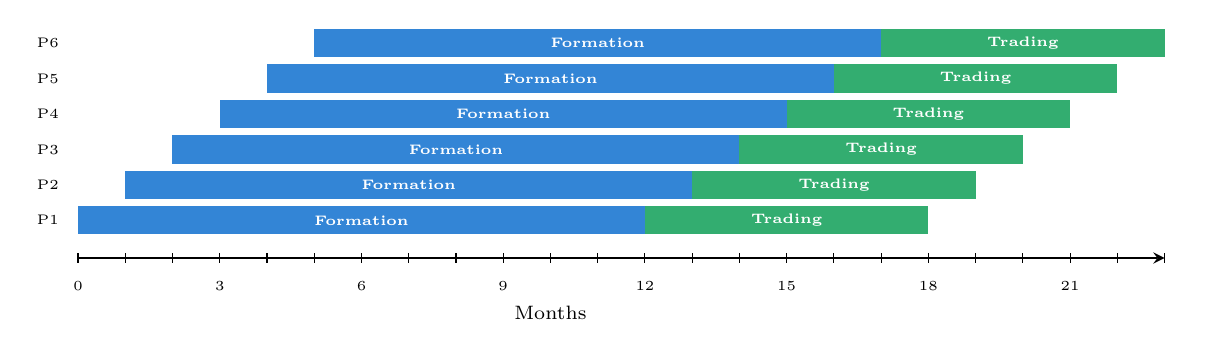
\begin{tikzpicture}[scale=0.6, font=\footnotesize]
  % Define colors
  \definecolor{formationcolor}{RGB}{0, 102, 204}
  \definecolor{tradingcolor}{RGB}{0, 153, 76}
  
  % Draw timeline axis
  \draw[thick, ->, >=stealth] (0,0) -- (23,0) node[right] {};
  
  % Draw month markers
  \foreach \x in {0,1,...,23} {
    \draw (\x,-0.1) -- (\x,0.1);
  }
  
  % Month labels
  \foreach \x/\label in {0/0,3/3,6/6,9/9,12/12,15/15,18/18, 21/21} {
    \node[below] at (\x,-0.3) {\tiny \label};
  }
  
  % Portfolio heights
  \def\pheight{0.6}
  \def\pgap{0.15}
  
  % Draw 6 portfolios
  \foreach \i in {1,...,6} {
    \pgfmathsetmacro\ystart{(\i-1)*(\pheight+\pgap)+0.5}
    \pgfmathsetmacro\xstart{\i-1}
    
    % Formation window
    \fill[formationcolor, opacity=0.8] (\xstart,\ystart) rectangle (\xstart+12,\ystart+\pheight);
    \node[white, font=\tiny\bfseries] at (\xstart+6,\ystart+\pheight/2) {Formation};
    
    % Trading window
    \fill[tradingcolor, opacity=0.8] (\xstart+12,\ystart) rectangle (\xstart+18,\ystart+\pheight);
    \node[white, font=\tiny\bfseries] at (\xstart+15,\ystart+\pheight/2) {Trading};
    
    % Labels
    \node[left] at (-0.2,\ystart+\pheight/2) {\tiny P\i};
  }
  
  % Month label
  \node[below] at (10,-0.8) {\scriptsize Months};
  
\end{tikzpicture}

\end{frame}

\section{Results}
%%%%%%%%%%%%%%%%%%%%%%%%%%%%%%%%%%%%%%%%%%%%%%%%%%%%%
\begin{frame}{Number of constituents in the replicating portfolio}
\begin{figure}[H]
  \centering
%  \caption{\textbf{Number of constituents in the replicating portfolio}}
  \includegraphics[scale=0.4]{/Users/jesusvillotamiranda/Library/CloudStorage/OneDrive-UniversidaddeLaRioja/GitHub/Repository/pairs_trading_sparse_synthetic_replica/__OUTPUT__/figures/distribution_of_nnz_w.pdf}
  \label{fig:}
\end{figure}
\end{frame}

%%%%%%%%%%%%%%%%%%%%%%%%%%%%%%%%%%%%%%%%%%%%%%%%%%%%%
\begin{frame}{Open pairs over time}
\begin{figure}[H]
%  \caption{\textbf{Number of Open Pairs}}
  \centering
  \includegraphics[scale=0.4]{/Users/jesusvillotamiranda/Library/CloudStorage/OneDrive-UniversidaddeLaRioja/GitHub/Repository/pairs_trading_sparse_synthetic_replica/__OUTPUT__/figures/num_open_pairs.pdf}
  \label{fig:}
\end{figure}
\end{frame}

%%%%%%%%%%%%%%%%%%%%%%%%%%%%%%%%%%%%%%%%%%%%%%%%%%%%%
\begin{frame}{Monthly Excess Return Distribution [no watiting]}
\begin{table}[H]
\centering
%\caption{\textbf{Monthly excess return distribution (no waiting)}}
\label{tab:excess_returns}
\footnotesize
\begin{tabular}{lcccc}
\toprule
Pairs portfolio & Top 5 & Top 20 & Pairs 101-120 & All Pairs \\
\midrule
%\textbf{A. Excess return distribution (no waiting)} & & & & \\
Average excess return (fully invested) & 0.01013 & 0.00971 & 0.01013 & 0.00859 \\
Standard error (Newey-West) & 0.00135 & 0.00103 & 0.00112 & 0.00074 \\
\textit{t}-Statistic & 7.50 & 9.39 & 9.01 & 11.59 \\
Excess return distribution & & & & \\
\quad Median & 0.00891 & 0.00871 & 0.01003 & 0.00826 \\
\quad Standard deviation & 0.03661 & 0.02511 & 0.02726 & 0.01873 \\
\quad Skewness & 0.49 & -0.10 & -0.32 & -0.25 \\
\quad Kurtosis & 4.47 & 4.90 & 7.96 & 17.44 \\
\quad Minimum & -0.09500 & -0.14352 & -0.18062 & -0.16669 \\
\quad Maximum & 0.18704 & 0.09846 & 0.17219 & 0.12407 \\
\quad Observations with excess return $<$ 0 & 39\% & 35\% & 32\% & 27\% \\
Average excess return on committed capital & 0.00644 & 0.00513 & 0.00499 & 0.00294 \\
\bottomrule
\end{tabular}

\medskip 
\textit{Period:} January 1963 to December 2024
\end{table}
\end{frame}

%%%%%%%%%%%%%%%%%%%%%%%%%%%%%%%%%%%%%%%%%%%%%%%%%%%%%
\begin{frame}{Monthly Excess Return Distribution [1 day watiting]}
\begin{table}[H]
\centering
%\caption{\textbf{Monthly excess return distribution (1 day waiting)}}
\label{tab:excess_returns}
\footnotesize
\begin{tabular}{lcccc}
\toprule
Pairs portfolio & Top 5 & Top 20 & Pairs 101-120 & All Pairs \\
\midrule
%\textbf{B. Excess return distribution (one day waiting)} & & & & \\
Average monthly return (fully invested) & 0.00853 & 0.00883 & 0.00854 & 0.00745 \\
Standard error (Newey-West) & 0.00129 & 0.00099 & 0.00113 & 0.00068 \\
\textit{t}-Statistic & 6.60 & 8.95 & 7.58 & 10.94 \\
Excess return distribution & & & & \\
\quad Median & 0.00650 & 0.00895 & 0.00863 & 0.00711 \\
\quad Standard deviation & 0.03714 & 0.02494 & 0.02726 & 0.01828 \\
\quad Skewness & 0.72 & -0.03 & -0.71 & -0.18 \\
\quad Kurtosis & 6.23 & 5.57 & 12.28 & 18.20 \\
\quad Minimum & -0.10801 & -0.15005 & -0.19062 & -0.16497 \\
\quad Maximum & 0.22563 & 0.10843 & 0.18429 & 0.12462 \\
\quad Observations with excess return $<$ 0 & 41\% & 36\% & 35\% & 30\% \\
Average excess return on committed capital & 0.00533 & 0.00440 & 0.00426 & 0.00250 \\
\bottomrule
\end{tabular}

\medskip 
\textit{Period:} January 1963 to December 2024
\end{table}
\end{frame}

%%%%%%%%%%%%%%%%%%%%%%%%%%%%%%%%%%%%%%%%%%%%%%%%%%%%%
\begin{frame}{Monthly excess returns [1 day waiting rule] (60 month rolling average)}
\begin{figure}[H]
%  \caption{\textbf{60-month rolling monthly excess returns}}
  \centering
  \includegraphics[scale=0.4]{/Users/jesusvillotamiranda/Library/CloudStorage/OneDrive-UniversidaddeLaRioja/GitHub/Repository/pairs_trading_sparse_synthetic_replica/__OUTPUT__/figures/comparison.pdf}
  \label{fig:}
\end{figure}
\end{frame}

%%%%%%%%%%%%%%%%%%%%%%%%%%%%%%%%%%%%%%%%%%%%%%%%%%%%%
\begin{frame}{Robustness to $\lambda$}
\textcolor{blue}{Blue: Replicating Portfolios for different $\lambda$ values} \\
\textcolor{red}{Red: Traditional Pairs Trading}
\begin{figure}[H]
%  \caption{Equity curve since 1990}
  \centering
  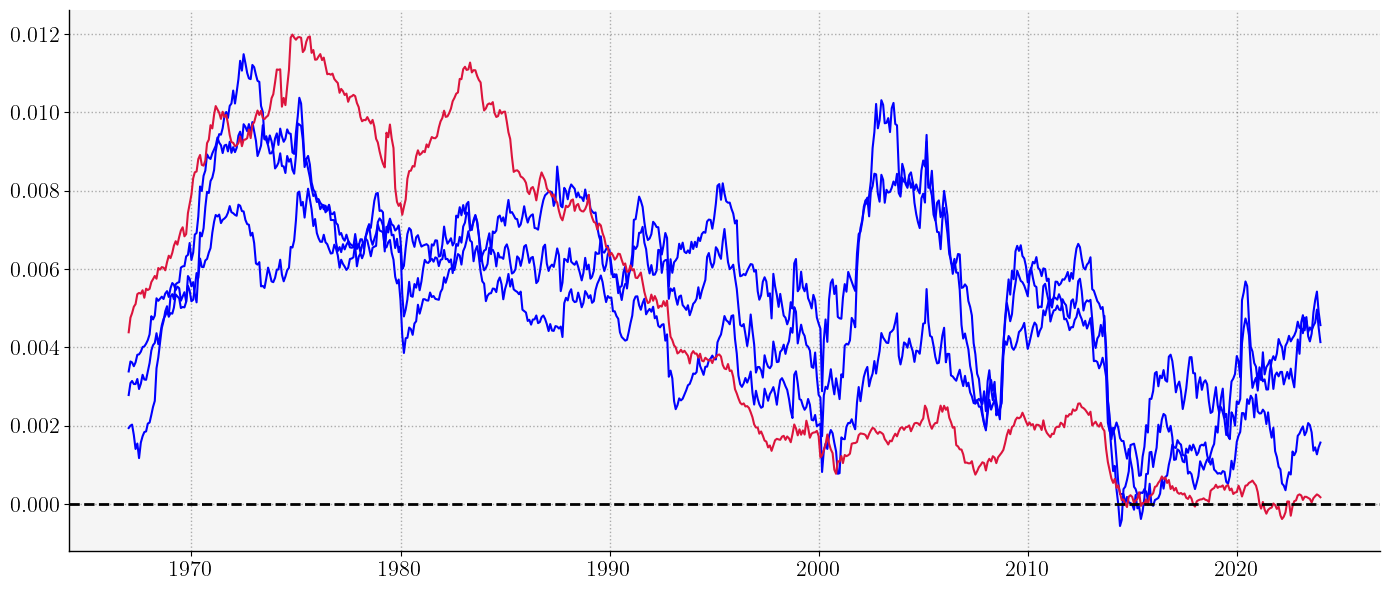
\includegraphics[scale=0.35]{/Users/jesusvillotamiranda/Library/CloudStorage/OneDrive-UniversidaddeLaRioja/GitHub/Repository/pairs_trading_sparse_synthetic_replica/__OUTPUT__/figures/robustness.pdf}
  \label{fig:}
\end{figure}
\end{frame}

%%%%%%%%%%%%%%%%%%%%%%%%%%%%%%%%%%%%%%%%%%%%%%%%%%%%%
\begin{frame}{Systematic Risk decomposition: FF5 + Reversals [1 day waiting]}
%\begin{table}[H]
\centering
\caption{Systematic risk of pairs trading strategies}
\label{tab:systematic_risk}
\footnotesize 
\begin{tabular}{lcccc}
\toprule
 & Top 5 & Top 20 & 20 after top 100 & All \\
\midrule
%\textit{``Wait one day'' portfolio performance} & & & & \\
%Mean excess return & 0.00853 & 0.00883 & 0.00854 & 0.00745 \\
%Standard deviation & 0.03714 & 0.02494 & 0.02726 & 0.01828 \\
%Sharpe Ratio & 0.80 & 1.23 & 1.08 & 1.41 \\
%Monthly serial correlation & -0.03 & 0.02 & 0.02 & 0.02 \\
%\\
%\textit{FF5 + Reversals} & & & & \\ \midrule
Intercept & 0.00618 & 0.00551 & 0.00525 & 0.00409 \\
 & \tiny(4.31) & \tiny(5.55) & \tiny(4.46) & \tiny(6.19) \\
\\[-0.5em]
Market & -0.15365 & -0.07676 & -0.06021 & -0.01491 \\
 & \tiny(-3.68) & \tiny(-3.12) & \tiny(-2.21) & \tiny(-0.76) \\
\\[-0.5em]
SMB & -0.06277 & -0.13786 & -0.21888 & -0.08163 \\
 & \tiny(-1.27) & \tiny(-2.97) & \tiny(-3.13) & \tiny(-1.51) \\
\\[-0.5em]
HML & -0.13321 & 0.03773 & 0.00239 & -0.01717 \\
 & \tiny(-1.75) & \tiny(0.77) & \tiny(0.04) & \tiny(-0.41) \\
\\[-0.5em]
Momentum & -0.09301 & -0.06905 & -0.14525 & -0.17550 \\
 & \tiny(-2.43) & \tiny(-2.19) & \tiny(-4.82) & \tiny(-8.36) \\
\\[-0.5em]
Short-Term Reversal & 0.15247 & 0.18033 & 0.23888 & 0.23198 \\
 & \tiny(2.67) & \tiny(4.37) & \tiny(4.83) & \tiny(6.26) \\
\\[-0.5em]
Long-Term Reversal & -0.01133 & -0.07164 & 0.05008 & -0.01632 \\
 & \tiny(-0.16) & \tiny(-1.26) & \tiny(0.84) & \tiny(-0.42) \\
\\[-0.5em]
$R^2$ & 0.05 & 0.11 & 0.19 & 0.41 \\
\bottomrule
\end{tabular}
\end{table}
\begin{table}[H]
\centering
%\caption{\textbf{Systematic risk of pairs trading strategies (1 day waiting)}}
\label{tab:systematic_risk}
\footnotesize
\begin{tabular}{lcccc}
\toprule
 & Top 5 & Top 20 & 20 after top 100 & All \\
\midrule
Mean excess return & 0.0085 & 0.0088 & 0.0085 & 0.0074 \\
Standard deviation & 0.0371 & 0.0249 & 0.0273 & 0.0183 \\
Sharpe Ratio & 0.80 & 1.23 & 1.08 & 1.41 \\
%Monthly serial corr. & -0.03 & 0.02 & 0.02 & 0.02 \\
\\ \textit{FF5+Reversals} &&&& \\ \midrule
\rowcolor{yellow!20}
Intercept & 0.0062 (4.31) & 0.0055 (5.55) & 0.0052 (4.46) & 0.0041 (6.19) \\
Market & -0.1537 (-3.68) & -0.0768 (-3.12) & -0.0602 (-2.21) & -0.0149 (-0.76) \\
SMB & -0.0628 (-1.27) & -0.1379 (-2.97) & -0.2189 (-3.13) & -0.0816 (-1.51) \\
HML & -0.1332 (-1.75) & 0.0377 (0.77) & 0.0024 (0.04) & -0.0172 (-0.41) \\
\rowcolor{yellow!20}
Momentum & -0.0930 (-2.43) & -0.0691 (-2.19) & -0.1452 (-4.82) & -0.1755 (-8.36) \\
\rowcolor{yellow!20}
Short-Term Reversal & 0.1525 (2.67) & 0.1803 (4.37) & 0.2389 (4.83) & 0.2320 (6.26) \\
Long-Term Reversal & -0.0113 (-0.16) & -0.0716 (-1.26) & 0.0501 (0.84) & -0.0163 (-0.42) \\ \midrule
$R^2$ & 0.05 & 0.11 & 0.19 & 0.41 \\
\bottomrule
\end{tabular}

\medskip 
\textit{Period:} January 1963 to December 2024
\end{table}
\end{frame}

%%%%%%%%%%%%%%%%%%%%%%%%%%%%%%%%%%%%%%%%%%%%%%%%%%%%%
\begin{frame}[label=equity00]{Equity curve to Pairs Trading since 2000}
%\hyperlink{equity90}{\beamergotobutton{Since 1990}}
\begin{figure}[H]
%  \caption{Equity curve from Pairs Trading since 2000}
  \centering
  \includegraphics[scale=0.35]{/Users/jesusvillotamiranda/Library/CloudStorage/OneDrive-UniversidaddeLaRioja/GitHub/Repository/pairs_trading_sparse_synthetic_replica/__OUTPUT__/figures/equity_curve_2000.pdf}
  \label{fig:}
\end{figure}
\end{frame}


%%%%%%%%%%%%%%%%%%%%%%%%%%%%%%%%%%%%%%%%%%%%%%%%%%%%%
\begin{frame}[label=equity90]{Equity curve since 1990}
%\hyperlink{equity00}{\beamergotobutton{Back}}
\begin{figure}[H]
%  \caption{Equity curve since 1990}
  \centering
  \includegraphics[scale=0.35]{/Users/jesusvillotamiranda/Library/CloudStorage/OneDrive-UniversidaddeLaRioja/GitHub/Repository/pairs_trading_sparse_synthetic_replica/__OUTPUT__/figures/equity_curve_1990.pdf}
  \label{fig:}
\end{figure}
\end{frame}

%%%%%%%%%%%%%%%%%%%%%%%%%%%%%%%%%%%%%%%%%%%%%%%%%%%%%
\begin{frame}[label=equity90]{Equity curve since 1963}
%\hyperlink{equity00}{\beamergotobutton{Back}}
%Had I invested 1\$ in Jan. 163... how much would I have in Dec. 2024?
\begin{figure}[H]
%  \caption{Equity curve since 1990}
  \centering
  \includegraphics[scale=0.35]{/Users/jesusvillotamiranda/Library/CloudStorage/OneDrive-UniversidaddeLaRioja/GitHub/Repository/pairs_trading_sparse_synthetic_replica/__OUTPUT__/figures/equity_curve_1963.pdf}
  \label{fig:}
\end{figure}
\end{frame}


\section{Conclusions}

%%%%%%%%%%%%%%%%%%%%%%%%%%%%%%%%%%%%%%%%%%%%%%%%%%%%%
\begin{frame}{Methodological Contributions}
\begin{itemize}
    \item \textcolor{blue}{\textbf{Conceptual advancement}}: We reframe pairs trading from a \textcolor{red}{rigid cardinality-constrained problem} to a \textcolor{DartmouthGreen}{flexible replicating portfolio framework}
    
    \bigskip
    \item \textcolor{blue}{\textbf{Practical implementation}}: LASSO regularization creates \textcolor{DartmouthGreen}{manageable portfolios} ($\approx$15 constituents) while maintaining superior replication quality
    
    \bigskip
    \item \textcolor{blue}{\textbf{Theoretical consistency}}: The approach preserves the \textcolor{DartmouthGreen}{fundamental economic intuition of relative-value arbitrage} while expanding the opportunity set
\end{itemize}
\end{frame}

%%%%%%%%%%%%%%%%%%%%%%%%%%%%%%%%%%%%%%%%%%%%%%%%%%%%%
\begin{frame}{Key Takeaway}

\medskip 
\begin{center}
\colorbox{DartmouthGreen!20}{%
    \begin{minipage}{0.75\textwidth}
        \centering
\textbf{Relative-value arbitrage is not obsolete (yet)}
    \end{minipage}
}
\end{center}

\bigskip 

\begin{itemize}

    \item \textbf{Traditional pairs trading's profitability has steadily declined since the 1990s}, confirming the decay documented in prior literature.
    
     \medskip
    \item The issue is \textbf{methodological limitation}: flexibility in substitute construction restores profitability
    
    \medskip
    \item \textbf{The replicating portfolio approach successfully revitalizes the strategy} by relaxing the restrictive 1-to-1 pairing constraint

%	 \item The \textbf{relative-value arbitrage principle} is as valid today as it was in the 1980s
%    \item What needed updating was the \textbf{methodological framework}, not the economic theory

	\medskip 
    \item Our approach offers a \textbf{principled path forward} for pairs trading in efficient markets
    
    
%    \medskip
%    \item \textbf{Sparse synthetic replicas outperform traditional pairs} across multiple performance metrics, generating positive risk-adjusted returns even in recent periods
\end{itemize}
\end{frame}



%%%%%%%%%%%%%%%%%%%%%%%%%%%%%%%%%%%%%%%%%%%%%%%%%%%%%%
%\begin{frame}{Market Implications}
%\begin{itemize}
%    \item \textcolor{DartmouthGreen}{\textbf{Pairs trading is not obsolete}} -- the underlying principle of relative pricing remains valid
%    
%    \medskip
%    \item \textcolor{DartmouthGreen}{\textbf{The issue was methodological limitation}}
%    
%    \medskip
%    \item \textcolor{DartmouthGreen}{\textbf{Flexibility in substitute construction}} can restore profitability to pairs trading
%    
%%    \medskip
%%    \item \textcolor{DartmouthGreen}{\textbf{Transaction costs remain manageable}} with sparse portfolio construction
%\end{itemize}
%\end{frame}


%%%%%%%%%%%%%%%%%%%%%%%%%%%%%%%%%%%%%%%%%%%%%%%%%%%%%%
%\begin{frame}{Bottom Line}
%\begin{center}
%\colorbox{DartmouthGreen!20}{%
%    \begin{minipage}{0.95\textwidth}
%        \centering
%        \textcolor{DartmouthGreen}{\textbf{Key Takeaway}}: By generalizing from \textbf{1-to-1} to \textbf{1-to-portfolio} relationships, we demonstrate that the fundamental insights of pairs trading remain \textbf{profitable in modern markets}
%    \end{minipage}
%}
%\end{center}
%
%\bigskip
%\begin{itemize}
%    \item The \textbf{relative-value arbitrage principle} is as valid today as it was in the 1980s
%    \item What needed updating was the \textbf{methodological framework}, not the economic theory
%    \item Our approach offers a \textbf{principled path forward} for pairs trading in efficient markets
%\end{itemize}
%\end{frame}

%%%%%%%%%%%%%%%%%%%%%%%%%%%%%%%%%%%%%%%%%%%%%%%%%%%%%%
%\begin{frame}{What about transaction costs?}
%\begin{itemize}
%	\item Is this strategy really feasible in practice?
%	\item Yes... If you are a hedge fund or an investment bank
%	\item No... for the mortal (unluckily, we in this room) 
%\end{itemize}
%\end{frame}

%%%%%%%%%%%%%%%%%%%%%%%%%%%%%%%%%%%%%%%%%%%%%%%%%%%%%
\begin{frame}[allowframebreaks]{References}
\bibliographystyle{apalike}
%\bibliographystyle{plainnat}  % Changed from 'plain'
\bibliography{bib_ref}
\end{frame}

%----------------------------------------------------
%%%%%%%%%%%%%%%%%%%%%%%%%%%%%%%%%%%%%%%%%%%%%%%%%%%%%
%%%%%%%%%%%%%%%%%%%%%%%%%%%%%%%%%%%%%%%%%%%%%%%%%%%%%
%%%%%%%%%%%%%%%%%%%%%%%%%%%%%%%%%%%%%%%%%%%%%%%%%%%%%
%%%%%%%%%%%%%%%%%%%%%%%%%%%%%%%%%%%%%%%%%%%%%%%%%%%%%
%----------------------------------------------------

%\appendix
%\section{Appendix}



\end{document}